\documentclass[nooutcomes]{ximera}
%% handout
%% space
%% newpage
%% numbers
%% nooutcomes

%I added the commands here so that I would't have to keep looking them up
%\newcommand{\RR}{\mathbb R}
%\renewcommand{\d}{\,d}
%\newcommand{\dd}[2][]{\frac{d #1}{d #2}}
%\renewcommand{\l}{\ell}
%\newcommand{\ddx}{\frac{d}{dx}}
%\everymath{\displaystyle}
%\newcommand{\dfn}{\textbf}
%\newcommand{\eval}[1]{\bigg[ #1 \bigg]}

%\begin{image}
%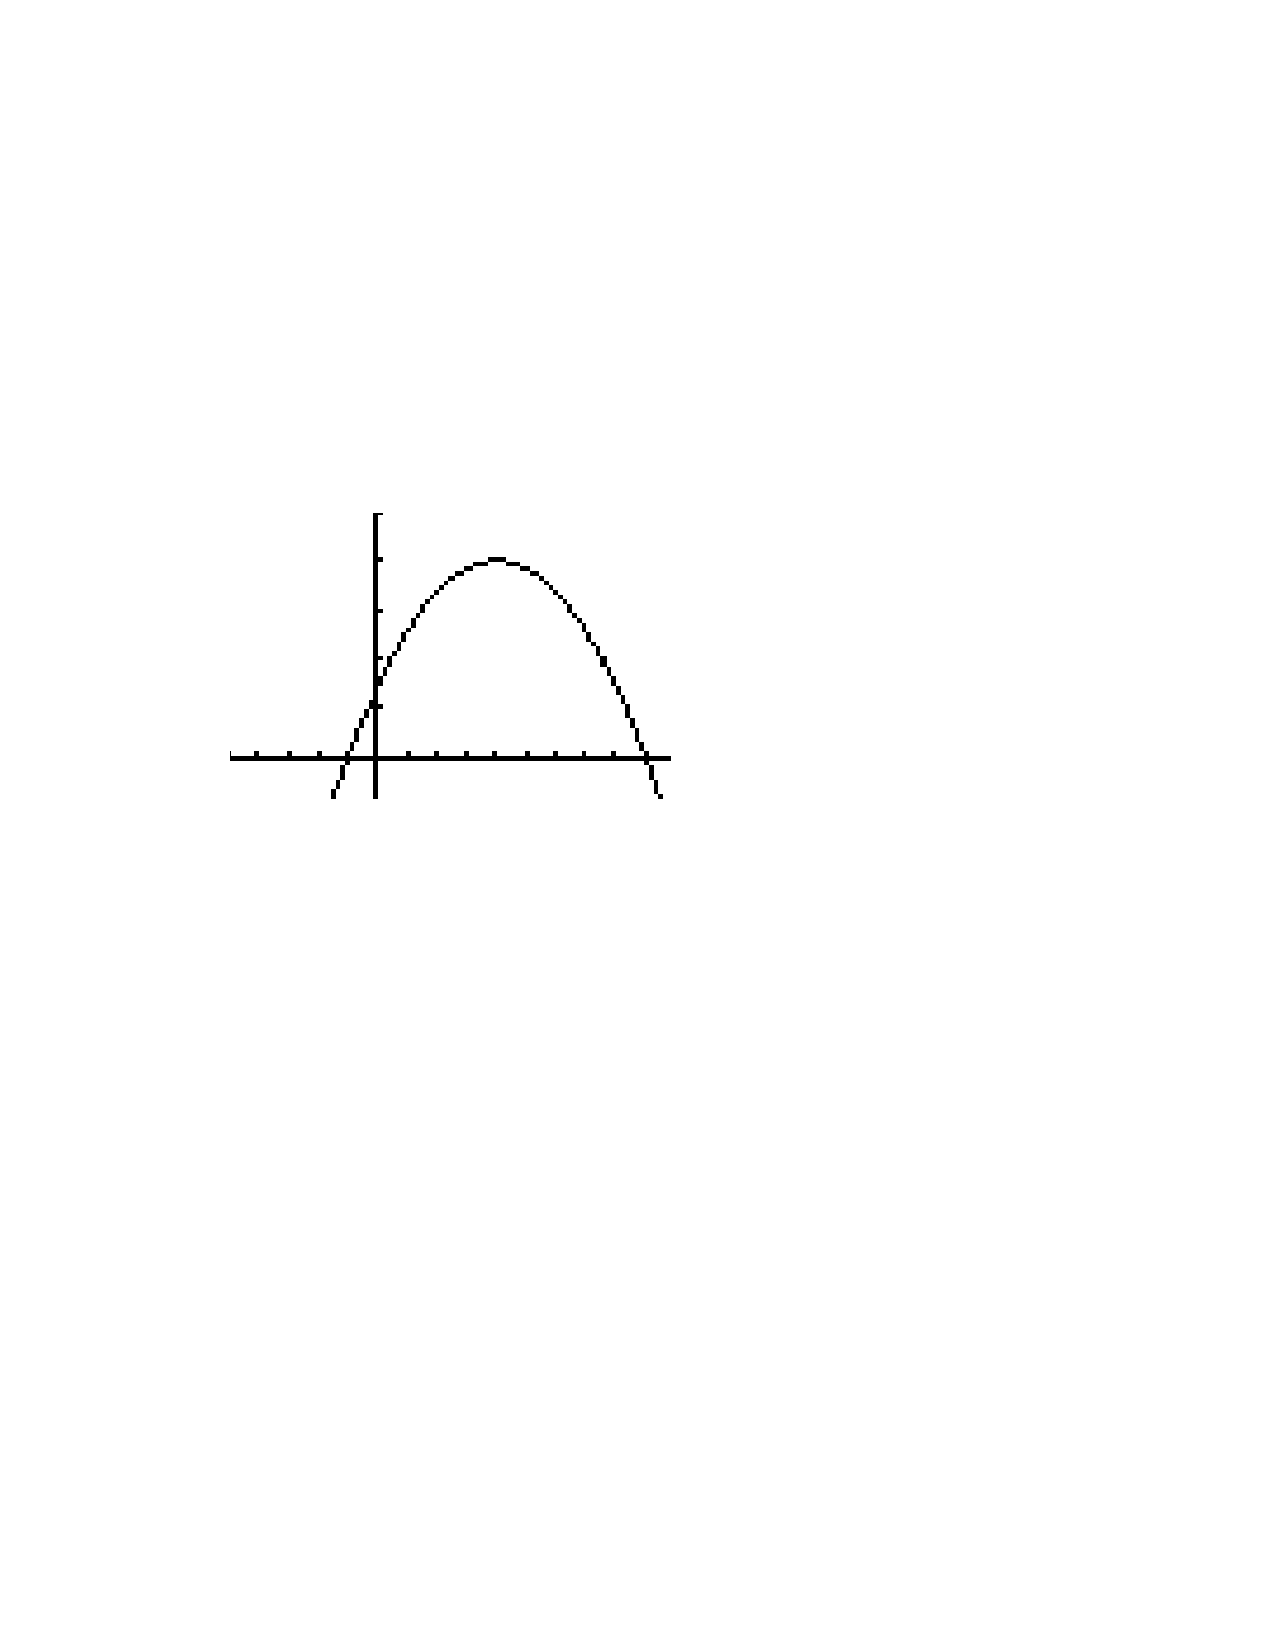
\includegraphics[trim= 170 420 250 180]{Figure1.pdf}
%\end{image}

\usepackage{fullpage}
\newcommand{\RR}{\mathbb R}
\renewcommand{\d}{\,d}
\newcommand{\dd}[2][]{\frac{d #1}{d #2}}
\renewcommand{\l}{\ell}
\newcommand{\ddx}{\frac{d}{dx}}
\newcommand{\dfn}{\textbf}
\newcommand{\eval}[1]{\bigg[ #1 \bigg]}

\usepackage{multicol}

\renewenvironment{freeResponse}{
\ifhandout\setbox0\vbox\bgroup\else
\begin{trivlist}\item[\hskip \labelsep\bfseries Solution:\hspace{2ex}]
\fi}
{\ifhandout\egroup\else
\end{trivlist}
\fi} %% we can turn off input when making a master document

\title{3.9: Derivatives of exponential and logarithmic functions}  

\begin{document}
\begin{abstract}		\end{abstract}
\maketitle

%problem1
\begin{problem}
  True or False:
  \begin{enumerate}
    \item[(1)]
      If $f(x) = (x-2)^x$, then $f'(x) = x (x-2)^{x-1}$.
      \begin{freeResponse}
        False.
        Any time that you have a function of $x$ raised to a function of $x$, in order to compute the derivative you need to use logarithmic differentiation (or something equivalent).

        Correct derivative of $f$:
        \begin{align*}
          f(x) &= (x-2)^x \implies f(x) = e^{x \ln(x-2)} \\
          &\implies f'(x) = e^{x \ln(x-2)} \cdot \left(1\cdot\ln(x-2) + x \cdot \frac{1}{x-2}\right) \\
          &\implies f'(x) = (x-2)^x \cdot \left(\ln(x-2) + \frac{x}{x-2}\right)
        \end{align*}
        \end{freeResponse}	
		
      \item[(2)]
        If $f(x) = (3x)^x$, then $f'(x) = (3x)^x \ln (3x)$.
	\begin{freeResponse}
          False.  Same as part (1).

          Correct derivative of $f$:
          \begin{align*}
            f(x) &= (3x)^x \implies f(x) = e^{x \cdot \ln(3x)} \\
            &\implies f'(x)  = e^{x \cdot \ln(3x)} \left(1 \cdot \ln(3x) + x \cdot \frac{3}{3x} \right) \\
            &\implies f'(x)  = (3x)^x \left(\ln(3x) + 1 \right)
          \end{align*}
	\end{freeResponse}	
	\end{enumerate}
\end{problem}

%problem2
\begin{problem}
Find the derivatives of the following functions:
	\begin{enumerate}
	
	%part a
	\item  $f(x) = x^{e^x} + 7x$
		\begin{freeResponse}
		$f'(x) = \ddx \left(x^{e^x} \right) + \ddx(7x) = \ddx \left(x^{e^x} \right) + 7$.  So the real problem is to find $\ddx \left(x^{e^x} \right)$.  
		
		\begin{align*}
		\ddx \left( x^{e^x} \right) &= \ddx \left( e^{\ln x^{e^x}} \right) \\
		&= \ddx \left( e^{e^x \ln x} \right) \\
		&= e^{e^x \ln x} \left( e^x \ln x + \frac{e^x}{x} \right) \\
		&= x^{e^x} \left( e^x \ln x + \frac{e^x}{x} \right).
		\end{align*}
		
		Thus, $f'(x) = x^{e^x} \left( e^x \ln x + \frac{e^x}{x} \right) + 7$.  
		
		\end{freeResponse}

	\item  $g(x) = (\ln x + 9)^{\sec(x^4)}$
		\begin{freeResponse}
			\begin{align*}
			g'(x) &= \ddx \left( (\ln x + 9)^{\sec(x^4)} \right) \\
			&= \ddx \left( e^{\sec(x^4) \ln ( \ln x + 9) } \right) \\
			&= e^{\sec(x^4) \ln ( \ln x + 9)} \left( 4x^3 \sec(x^4) \tan(x^4) \ln(\ln x + 9) + \sec(x^4) \frac{\frac{1}{x}}{\ln x + 9} \right) \\
			&= (\ln x + 9)^{\sec(x^4)} \left( 4x^3 \sec(x^4) \tan(x^4) \ln(\ln x + 9) + \frac{\sec(x^4)}{x(\ln x + 9)} \right) .
			\end{align*}
		\end{freeResponse}
		
	%part c
	\item  $h(x) = \frac{(x^2 - 7)^5}{\cos^7(x^2 - 5)}$
          \begin{freeResponse}
            Rewrite $h(x)$ using properties of logarithms:
            \begin{align*}
              \ln h(x) &= \ln \left( \frac{(x^2 - 7)^5}{\cos^7(x^2 - 5)}\right) \\
                       &= 5 \cdot \ln (x^2 - 7) + 7 \cdot \ln(\cos(x^2-5))
            \end{align*}
            % \begin{align*}
            %   h(x) &= e^{\ln(h(x))} = e^{\ln\left((x^2 - 7)^5/\cos^7(x^2 - 5)\right)}\\
            %   &= e^{\ln((x^2-7)^5) - \ln(\cos^7(x^2-5))} \\
            %   &= e^{5\cdot \ln((x^2-7)) - 7 \cdot \ln(\cos(x^2-5))}
            % \end{align*}

            Derivative of $h$:
            \begin{align*}
              \ddx \ln h(x) &\implies \frac{h'(x)}{h(x)} = 5 \cdot \frac{1}{x^2 - 7} \cdot 2x + 7 \cdot\frac{1}{\cos(x^2 - 5)} \cdot - \sin^2(x^2-5) \cdot 2x\\
                            &= \frac{10x}{x^2-7} - \frac{14x \cdot \sin(x^2 - 5)}{\cos(x^2 - 5)}\\
              &= \frac{10x}{x^2-7} - 14x \tan(x^2-5) \\
              &\implies h'(x) = h(x)\cdot \left( \frac{10x}{x^2-7} - 14x \tan(x^2-5) \right) \\
              &= h'(x) = \frac{(x^2 - 7)^5}{\cos^7(x^2 - 5)} \cdot \left( \frac{10x}{x^2-7} - 14x \tan(x^2-5) \right)
              % h(x) &= e^{5\cdot \ln((x^2-7)) - 7 \cdot \ln(\cos^7(x^2-5))}\\
              % &\implies h'(x) = e^{5\cdot \ln((x^2-7)) - 7 \cdot \ln(\cos(x^2-5))}\cdot \left(5\cdot \frac{1}{x^2-7} \cdot 2x - 7 \cdot -\sin(x^2-5)\cdot 2x \right) \\
              % &\implies h'(x) = h(x) \cdot \left( \frac{10x-35}{x^2-7} + 14x\sin(x^2-5)\right)
            \end{align*}
	\end{freeResponse}
	\end{enumerate}
\end{problem}






\end{document} 


















